% 4-5 pages total.

% Goals:
% Cover each aspect of evaluation and discussion of results.
% Software testing – strategy & statistics (1-2 pages).
% Explanation of evaluation strategy (1/2 page).
% Evaluation Results (1-2 pages).

% Marking:
% Has the software been thoroughly tested, and subjected to appropriate user evaluation? Does the student have good suggestions for further work?
% A-band: The evaluation is really thorough. There are excellent suggestions for further work.

\chapter{Testing \& Evaluation}\label{testing_evaluation}

\section{Testing}
% - Use of unit tests and CI.
% - Testing on VM for Windows.
% - Variety of Blender models to establish limits.

\subsection{Unit Testing}

Reliance of the System on the \texttt{bpy} module drove different testing strategies for the \texttt{view-controller} and \texttt{model}.
The separation of concerns provided by the chosen architecture was chosen in part to support robust automated testing.
First, tests related to the \texttt{model} (\texttt{bpy}-independent) are run within the local virtual environment.
Then, tests related to  the \texttt{view-controller} (\texttt{bpy}-dependent) are run within the Blender environment, using Blender's headless mode (\texttt{-b} flag).
Both strategies are combined in a bash script, which acts as the test runner.

\lstinputlisting[language=bash, caption=Unit test runner (run\_tests.sh).]{../run_tests.sh}

Automated testing within the \texttt{model} package focusses on functionality provided by foundational Classes in the \texttt{primitives} module.
These are tested as far as practical with unit tests. 
Any required input image data is mocked/stubbed by supplying simple \texttt{numpy} arrays.

Automated testing within \texttt{view-controller} covers aspects such as testing of add-on registration and GUI creation.

To ensure that tests are run frequently, and to prevent regressions in new commits, a Continuous Integration approach was taken.
The Travis service was used as a build server, and hooked into the project's GitHub repository.
The server was configured to first install all necessary Blender and Python dependencies, install the add-on, and then execute the test suites.

\lstinputlisting[caption=Travis configuration (.travis.yml).]{../.travis.yml}

\subsection{Validation Testing}

To ensure the System operated as expected with regards to basic functional requirements, a series of input Blender models were chosen for validation testing.
This consisted of a selection of mathematical surface models (the core-focus of the project), and a selection of assorted objects intended to test the flexibility and limits of the System.

Overall, the System performs very well, yielding high-quality SVG renderings for mathematical surfaces and assorted objects, which (to the author's eye) accurately conveys structure and character of the object. A subset rendered test scenes are presented in Appendix \ref{appendix_renders}. However, two bugs were identified which have not been addressed prior to submission, both are related to Silhouette lines.

First, silhouette lines fail to express the correct line thickness at the intersection of some internal edges. This is particularly visible when silhouette thickness is scaled according to depth when the silhouette spans two extreme depth values.

\begin{figure}[h!]
	\centering
	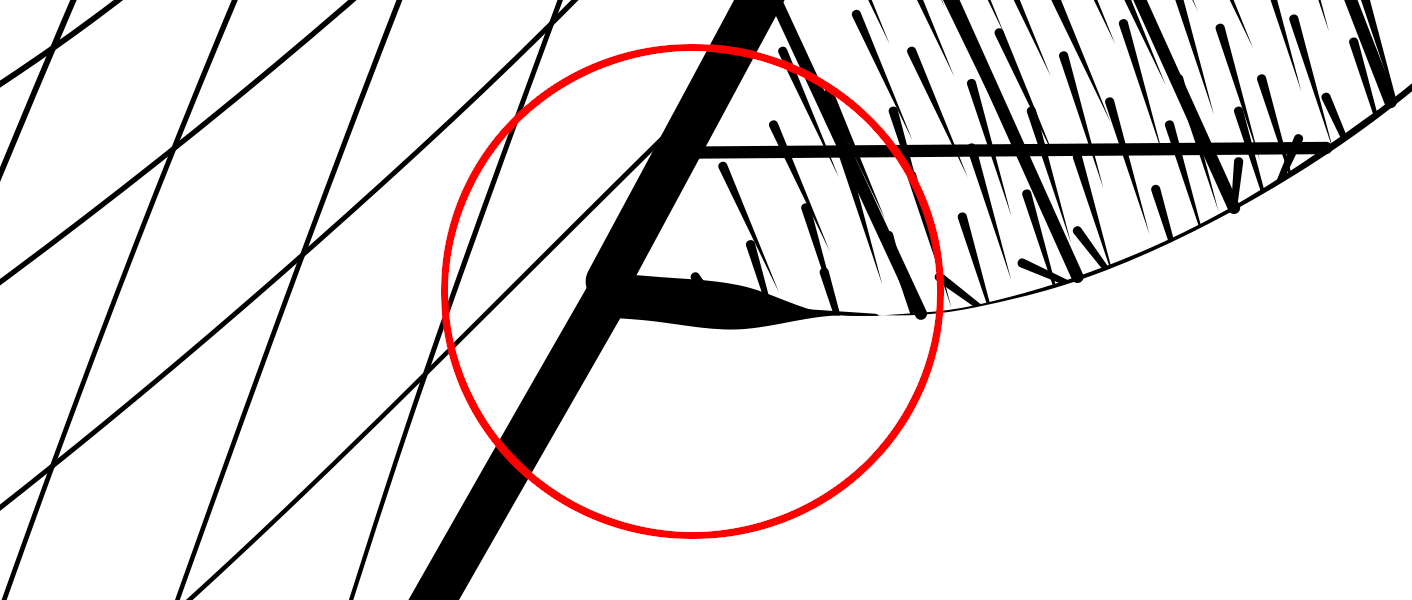
\includegraphics[width=\textwidth]{images/silhouette_bug.png}
	\caption{Extreme close-up of Figure \ref{render_hyperbolic_paraboloid_polar}, demonstrating silhouette bleed-over. The line leading to the right should be thin, to represent the relatively far distance of that edge from the camera. Instead it is rendered thick, because the value at the 3-way intersection is sampled for depth, which is relatively close to the camera.}\label{silhouette_bug}
\end{figure}

The issue demonstrated in Figure \ref{silhouette_bug} stems from the method used to construct \texttt{CurvedStroke}s. The value of interest (in this case intensity of the depth map) of the underlying surface is sampled in globally-fixed intervals along the length of a stroke. The line thickness is then scaled based on this underlying value.
This approach works well when the thickness varies gradually and linearly, however fails when very large changes must be reflected over small distances.
A simple solution is to greatly increase the sampling interval, however this will incur performance penalties.
A more intelligent approach may be appropriate, where areas of significant change are identified in pre-processing and the sampling interval is greatly increased only at these local areas.

The second issue is well-demonstrated by Figure \ref{render_brooklyn}, and to a lesser extent Figure \ref{render_taranaki}.
Both of these images are distinct from the others in that the render subject is not entirely contained within the scene.
The underlying \texttt{Silhouette} mechanism is extraction of a closed-path by \texttt{skimage.measure.find\_contours}.
Occasionally, \texttt{find\_contours} will locate multiple contours, and the System assumes that the longest path is the true silhouette.
When the silhouette leads off screen, we essentially have multiple silhouette paths.
A fix therefore would involve supporting these multiple silhouette paths, rather than discarding all but the longest.

\section{Evaluation}
% - Eval, rationale/aim. Results. Conclusions.

\subsection{Strategy}

To critically evaluate the System, an online survey was created\footnote{\url{https://www.surveylegend.com/s/xbk}} and distributed to a knowledgeable audience on \url{BlenderArtists.org}, and amongst fellow Computer Science students at the University of Glasgow.
Three key questions were asked, each requiring review of multiple renderings produced by the System.

\begin{enumerate}
	\item{Style: Comparison of styles, where the participant was asked to compare a simple render produced by Blender with two renders produced by the System, and indicate a ranked preference. 13 distinct objects were presented, rendered in these three different styles. See Figure \ref{eval_styles}.}
	\item{Parsimony of Ink: Evaluation of techniques for minimising ink usage, where the participant indicates the image which most effectively communicates critical features whilst also minimising ink use. A single object was presented, rendered in 6 different variations of System styles. See Figures \ref{eval_ink_1} and \ref{eval_ink_2}.}
	\item{Quality: Evaluation of overall quality, where renders were presented and the participant asked to rank each on a scale of 1-5 according to general quality and aesthetic value. 11 high-quality renderings were produced, aiming to showcase System ``best-effort''. See Figure \ref{eval_quality}.}
\end{enumerate}

The goal of the evaluation was to get an overall sense of the success of the System with regards to project goals, and to identify areas for further development.

\subsection{Results}

A total of 12 participants completed the survey, around half of whom were students at the University of Glasgow, and half forum members from \url{BlenderArtists.org}. A further 13 participants only partially completed the survey. As value can still be derived from these partial results, these are included in analysis.

\subsubsection{Style}

The objects presented were a mixture of mathematical surfaces and other assorted objects.
As the focus of the project is mathematical surfaces, results from each of these two categories are considered separately.

For each rendering of a given object, each participant voted whether it should be ranked 1st, 2nd, or 3rd in terms of preference. The measure was effectiveness of the image to convey structure and overall character of the object. Votes were collated and are presented in Appendix \ref{appendix_eval_results}, along with an explanation of process.

For mathematical images, a strong preference exists for the Streamline style.
This makes some sense, as the mathematical surfaces presented are continuous, allowing for surface streamlines to cleanly follow the underlying structure in a pleasing way.
Renderings produce by Blender (with a default diffuse material applied) and those produced by the System in the stipple style are tied for second preference.
Both of these styles rely on Blender's (Cycles') underlying lighting model to produce the appearance of shading, so this correlation makes some sense.
It is encouraging that the stipple style is viewed as effective as Blender's, and suggests that stipples can be used as alternative, with the added benefits that hand-drawn styles can bring.

Results from other objects are less clear cut, and suggest a moderate preference for Blender's style, followed by stipples, with streamlines lagging in third.
This may be due to the more complex discontinuous nature of these objects.
The relatively larger amounts of ink required of the Blender renders perhaps allows smaller details to be better communicated, however it may be possible to tweak the NPR styles to better imitate this, through use of denser stippling for example.
The subjectivity suggested by the results here makes it difficult to draw any firm conclusions however, and further work would useful to assess a wider range of objects with an increased number of participants.

\subsubsection{Parsimony of Ink}

The opportunity was taken at this point in the survey to gain a general awareness of how far ink usage can be minimised whilst still retaining an ability to convey the character of an object.

The approach taken was to render a series of images in a mixture of streamline and stipple styles. 
Images start out with very low ink usage (subtle styles), and gradually become more ink-heavy.
The general idea was that a point will be reached where just enough ink exists on the page to allow the object to be understood.
This insight can help future development, giving some basis to setting of sensible System defaults for example.
For each image, ink usage was given a ``cost'' (computed by summing the intensities of all pixels in a rasterised version of the SVG).
The goal was to allow the participant to select the image which communicates form, whilst also minimising this cost.

Results are presented in Appendix \ref{appendix_eval_results}. It appears that very low ink usage is possible - the most widely preferred style was streamlines with line thickness scaled according to line curvature.
This result suggests there is value to further development to improve this style of line expression.

\FloatBarrier
\subsubsection{Quality}

\begin{wrapfigure}{r}{0.3\textwidth}
  \begin{center}
    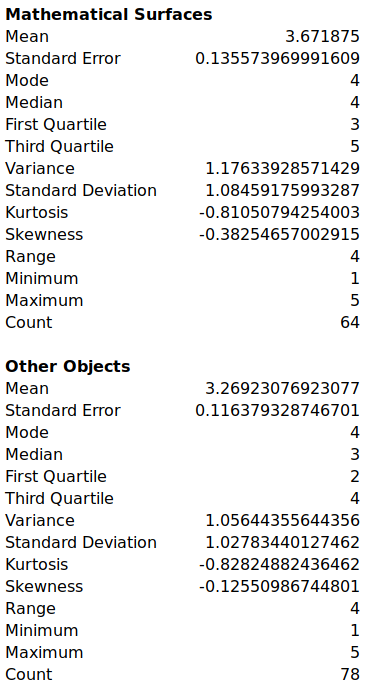
\includegraphics[scale=0.3]{images/eval_quality_results.png}
  \end{center}
  \caption{Statistics describing rendering quality ratings.}\label{eval_quality_results}
\end{wrapfigure}

Finally, the participant was asked to rate various renderings produced using different combinations of System styles, in a manner thought to best suit the individual object. This represents a ``best-effort'' showcase of images, the goal being to assess the general level of quality of the produced images.

Participants rated each image on a scale of 1 to 5, with 1 described as ``very poor'', and 5 described as ``superb''. 
Again, images are separated into two groups for analysis - mathematical surfaces and other objects.

Overall, mathematical surfaces are deemed to be rendered at a higher quality level, and some examples were consistently rated ``superb''.
Other objects do not perform as well, however results are still generally positive.

These are encouraging results, considering the short time-span of the project and the critical audience chosen.

% \begin{figure}[h!]
% 	\centering
% 	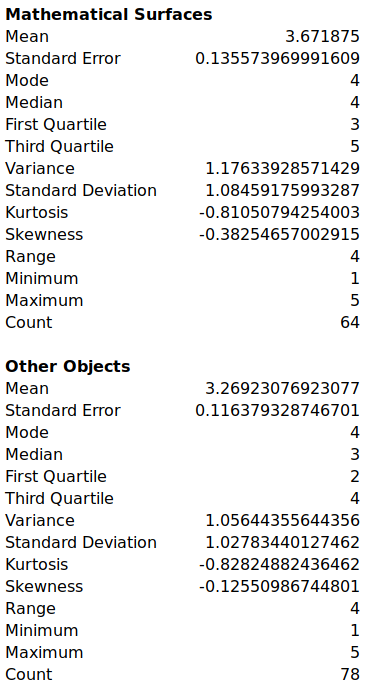
\includegraphics[scale=0.2]{images/eval_quality_results.png}
	
% \end{figure}